\PassOptionsToPackage{table}{xcolor}
\documentclass[12pt,letterpaper,twocolumn,openany,nodeprecatedcode,bg=none]{dndbook}
\usepackage[english]{babel}
\usepackage[utf8]{inputenc}
\usepackage{longtable,booktabs,array}
\usepackage{calc}
\usepackage{etoolbox}
\usepackage{caption}
\usepackage{float}
\usepackage{graphicx}
\usepackage{needspace}
\usepackage{tikz}

% Reset zebra striping at the start of every table
\AtBeginEnvironment{longtable}{\rowcolors{1}{white}{gray!10}\small}
\AtBeginEnvironment{table}{\rowcolors{1}{white}{gray!10}}

\providecommand{\pandocbounded}[1]{#1}
\providecommand{\tightlist}{%
  \setlength{\itemsep}{0pt}\setlength{\parskip}{0pt}}

\captionsetup{labelformat=empty}
\setcounter{secnumdepth}{0}
\setlength{\parindent}{0pt}
\setlength{\parskip}{0.5\baselineskip}
\setlength{\headheight}{15pt}

% Prevent orphaned subsections
\let\oldsubsection\subsection
\renewcommand{\subsection}[1]{%
  \needspace{5\baselineskip}%
  \oldsubsection{#1}%
}

\begin{document}
\onecolumn

      \title{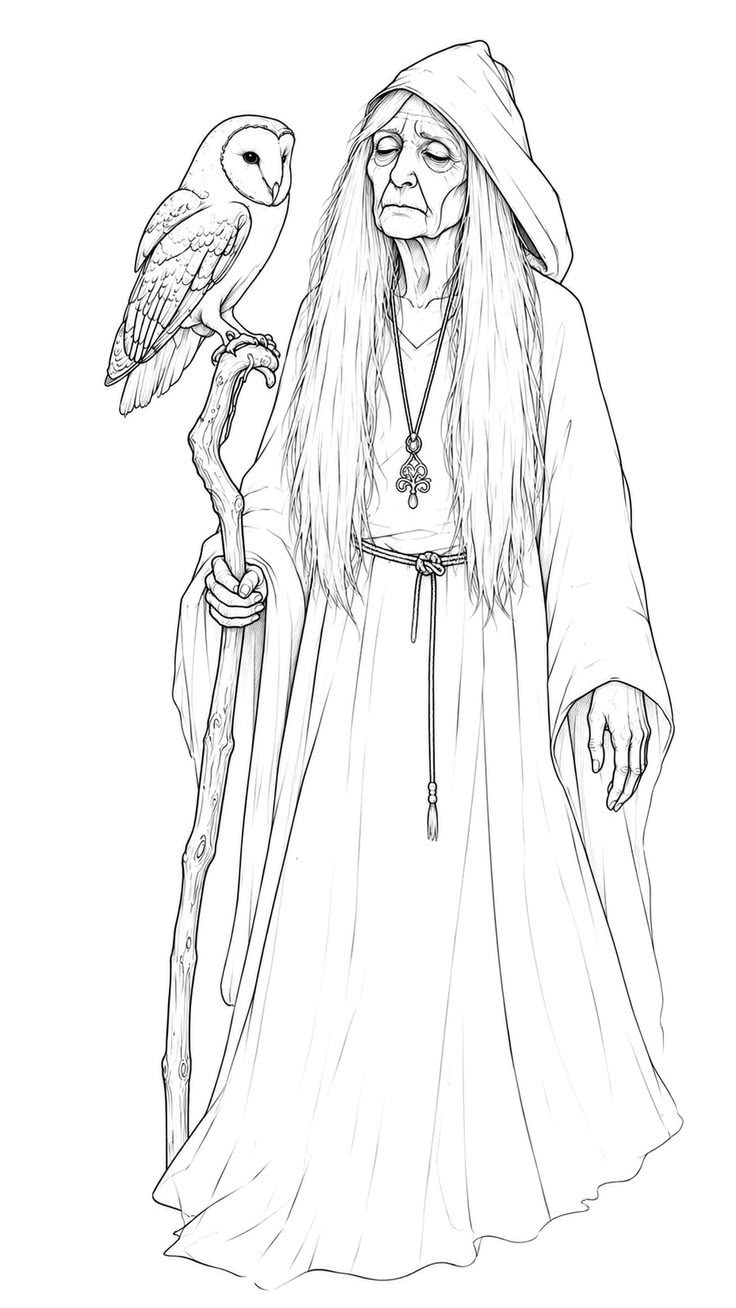
\includegraphics[width=0.9\textwidth,height=0.55\textheight,keepaspectratio]{oldWoman.jpg}\\[1.5cm]Mystic
of Life}
  \author{Class Handbook}
\date{}
\maketitle



\clearpage
\twocolumn

\section{Mystic (Life)}\label{mystic-life}

\subsection{Core Mystic (Life) Traits}\label{core-mystic-life-traits}

\needspace{11\baselineskip}

{\def\LTcaptype{none} % do not increment counter
\begin{table}[!htbp]
\centering
\begin{tabular}{@{}
  >{\raggedright\arraybackslash}p{(\linewidth - 2\tabcolsep) * \real{0.3095}}
  >{\raggedright\arraybackslash}p{(\linewidth - 2\tabcolsep) * \real{0.6905}}@{}}
\toprule\noalign{}
\begin{minipage}[b]{\linewidth}\raggedright
\textbf{Primary Ability}
\end{minipage} & \begin{minipage}[b]{\linewidth}\raggedright
Wisdom
\end{minipage} \\
\midrule\noalign{}
\textbf{Hit Points} & 1d6 \\
\textbf{Saving Throw Proficiencies} & Intelligence, Wisdom \\
\textbf{Skill Proficiencies} & Choose 2 skills \\
\textbf{Weapon Proficiencies} & Choose 2 categories \\
\textbf{Starting Equipment} & Mace, Dagger, Chain Mail, Open Helm,
Shield, Sacred Symbol \\
\bottomrule\noalign{}
\end{tabular}
\end{table}
}

\subsection{Mystic (Life) Features}\label{mystic-life-features}

\needspace{20\baselineskip}

{\def\LTcaptype{none} % do not increment counter
\begin{table}[!htbp]
\centering
\begin{tabular}{@{}
  >{\raggedright\arraybackslash}p{(\linewidth - 4\tabcolsep) * \real{0.1220}}
  >{\raggedright\arraybackslash}p{(\linewidth - 4\tabcolsep) * \real{0.2683}}
  >{\raggedright\arraybackslash}p{(\linewidth - 4\tabcolsep) * \real{0.6098}}@{}}
\toprule\noalign{}
\begin{minipage}[b]{\linewidth}\raggedright
Level
\end{minipage} & \begin{minipage}[b]{\linewidth}\raggedright
Proficiency
\end{minipage} & \begin{minipage}[b]{\linewidth}\raggedright
Class Features
\end{minipage} \\
\midrule\noalign{}
1 & +2 & Spellcasting, Turn Undead \\
2 & +2 & --- \\
3 & +2 & Ability Bonus \\
4 & +2 & --- \\
5 & +2 & --- \\
6 & +2 & --- \\
7 & +2 & Ability Bonus \\
8 & +2 & --- \\
9 & +3 & --- \\
10 & +3 & --- \\
\bottomrule\noalign{}
\end{tabular}
\end{table}
}

\subsection{Level 1: Spellcasting}\label{level-1-spellcasting}

You can cast spells from the Mystic (Life) spell list. Wisdom is your
casting ability. You know two cantrips.

You prepare a number of spells equal to your total number of spell
slots. You may change your prepared spells after an extended period of
downtime.

You regain all expended spell slots when you finish a long rest. Once
per day, you may regain 1 expended spell slot when you finish a short
rest.

\subsection{Spell Slots by Level}\label{spell-slots-by-level}

\needspace{20\baselineskip}

{\def\LTcaptype{none} % do not increment counter
\begin{table}[!htbp]
\centering
\begin{tabular}{@{}
  >{\raggedright\arraybackslash}p{(\linewidth - 6\tabcolsep) * \real{0.3571}}
  >{\raggedright\arraybackslash}p{(\linewidth - 6\tabcolsep) * \real{0.2143}}
  >{\raggedright\arraybackslash}p{(\linewidth - 6\tabcolsep) * \real{0.2143}}
  >{\raggedright\arraybackslash}p{(\linewidth - 6\tabcolsep) * \real{0.2143}}@{}}
\toprule\noalign{}
\begin{minipage}[b]{\linewidth}\raggedright
Level
\end{minipage} & \begin{minipage}[b]{\linewidth}\raggedright
1
\end{minipage} & \begin{minipage}[b]{\linewidth}\raggedright
2
\end{minipage} & \begin{minipage}[b]{\linewidth}\raggedright
3
\end{minipage} \\
\midrule\noalign{}
1 & 2 & -- & -- \\
2 & 2 & -- & -- \\
3 & 3 & -- & -- \\
4 & 3 & -- & -- \\
5 & 4 & 2 & -- \\
6 & 4 & 2 & -- \\
7 & 4 & 3 & -- \\
8 & 4 & 3 & -- \\
9 & 4 & 3 & 2 \\
10 & 4 & 3 & 2 \\
\bottomrule\noalign{}
\end{tabular}
\end{table}
}

\subsection{Level 1: Turn Undead}\label{level-1-turn-undead}

As an action, you present your sacred symbol. All undead within 30 feet
of you must make Wisdom saves opposed by your Wisdom check. If they
fail, they are frightened of you for 1 minute or until they take damage.
If they succeed, they are immune to your use of this feature for the
next 24 hours.

\subsection{Level 3: Ability Bonus}\label{level-3-ability-bonus}

You gain a +1 bonus to two different abilities of your choice.

\subsection{Level 7: Ability Bonus}\label{level-7-ability-bonus}

You gain a +1 bonus to two different abilities of your choice.

\newpage

\subsection{Mystic (Life) Spells}\label{mystic-life-spells}

The tables are numbered for random spell selection.

\subsubsection{Cantrips}\label{cantrips}

\needspace{13\baselineskip}

{\def\LTcaptype{none} % do not increment counter
\begin{table}[!htbp]
\centering
\begin{tabular}{@{}
  >{\raggedright\arraybackslash}p{(\linewidth - 2\tabcolsep) * \real{0.1667}}
  >{\raggedright\arraybackslash}p{(\linewidth - 2\tabcolsep) * \real{0.8333}}@{}}
\toprule\noalign{}
\begin{minipage}[b]{\linewidth}\raggedright
d6
\end{minipage} & \begin{minipage}[b]{\linewidth}\raggedright
Cantrip
\end{minipage} \\
\midrule\noalign{}
1 & Light \\
2 & Mending \\
3 & Sacred Flame \\
4 & Spare the Dying \\
5 & Thaumaturgy \\
6 & True Strike \\
\bottomrule\noalign{}
\end{tabular}
\end{table}
}

\subsubsection{Level 1 Spells}\label{level-1-spells}

\needspace{13\baselineskip}

{\def\LTcaptype{none} % do not increment counter
\begin{table}[!htbp]
\centering
\begin{tabular}{@{}
  >{\raggedright\arraybackslash}p{(\linewidth - 2\tabcolsep) * \real{0.1765}}
  >{\raggedright\arraybackslash}p{(\linewidth - 2\tabcolsep) * \real{0.8235}}@{}}
\toprule\noalign{}
\begin{minipage}[b]{\linewidth}\raggedright
d6
\end{minipage} & \begin{minipage}[b]{\linewidth}\raggedright
Level 1
\end{minipage} \\
\midrule\noalign{}
1 & Bless \\
2 & Command \\
3 & Cure Wounds \\
4 & Detect Magic \\
5 & Guiding Bolt \\
6 & Inflict Wounds \\
\bottomrule\noalign{}
\end{tabular}
\end{table}
}

\subsubsection{Level 2 Spells}\label{level-2-spells}

\needspace{13\baselineskip}

{\def\LTcaptype{none} % do not increment counter
\begin{table}[!htbp]
\centering
\begin{tabular}{@{}
  >{\raggedright\arraybackslash}p{(\linewidth - 2\tabcolsep) * \real{0.1500}}
  >{\raggedright\arraybackslash}p{(\linewidth - 2\tabcolsep) * \real{0.8500}}@{}}
\toprule\noalign{}
\begin{minipage}[b]{\linewidth}\raggedright
d6
\end{minipage} & \begin{minipage}[b]{\linewidth}\raggedright
Level 2
\end{minipage} \\
\midrule\noalign{}
1 & Augury \\
2 & Hold Creature \\
3 & Restorative Touch \\
4 & Silence \\
5 & Spectral Weapon \\
6 & Zone of Truth \\
\bottomrule\noalign{}
\end{tabular}
\end{table}
}

\newpage

\subsubsection{Level 3 Spells}\label{level-3-spells}

\needspace{13\baselineskip}

{\def\LTcaptype{none} % do not increment counter
\begin{table}[!htbp]
\centering
\begin{tabular}{@{}
  >{\raggedright\arraybackslash}p{(\linewidth - 2\tabcolsep) * \real{0.1200}}
  >{\raggedright\arraybackslash}p{(\linewidth - 2\tabcolsep) * \real{0.8800}}@{}}
\toprule\noalign{}
\begin{minipage}[b]{\linewidth}\raggedright
d6
\end{minipage} & \begin{minipage}[b]{\linewidth}\raggedright
Level 3
\end{minipage} \\
\midrule\noalign{}
1 & Dispel Magic \\
2 & Protection from Energy \\
3 & Remove Curse \\
4 & Revivify \\
5 & Speak with Dead \\
6 & Spirit Guardians \\
\bottomrule\noalign{}
\end{tabular}
\end{table}
}

\section{Mystic (Life) Spell List}\label{mystic-life-spell-list}

Spells descriptions are listed below.

\subsection{Augury}\label{augury}

\textbf{Level:} 2

You receive an omen from mystical forces about the results of a course
of action that you plan to take within the next 30 minutes. The DM
chooses whether to answer weal, woe, or a mix of the two, depending on
the most likely outcome of the action.

\subsection{Bless}\label{bless}

\textbf{Level:} 1

\textbf{Range:} 30 feet

\textbf{Duration:} Concentration, up to 1 minute

You bless up to three creatures within range. A blessed creature adds
1d4 to their attack rolls and saves.

\newpage

\subsection{Command}\label{command}

\textbf{Level:} 1

\textbf{Range:} 60 feet

You speak a one-word command to a creature in range. The target must
succeed on a Wisdom saving throw or follow the command on its next turn.
The DM adjudicates its actions, or you can choose one of these options:

\textbf{Approach.} The target moves toward you.

\textbf{Drop.} The target falls prone.

\textbf{Flee.} The target moves away from you.

\textbf{Halt.} On its turn, the target doesn't move.

You can use a higher-level spell slot to cast this spell. A level 2 slot
allows you to target two creatures and a level 3 one allows you to
target three creatures.

\subsection{Cure Wounds}\label{cure-wounds}

\textbf{Level:} 1

\textbf{Range:} Touch

A creature you touch regains 2d8 + your spellcasting bonus hit points.

The healing increases to 4d8 + your spellcasting bonus if you use a
level 2 slot and 6d8 + your spellcasting bonus if you use a level 3
slot.

\subsection{Detect Magic}\label{detect-magic}

\textbf{Level:} 1

\textbf{Range:} Self

\textbf{Duration:} Concentration, up to 10 minutes

You see the presence of magical effects within 30 feet on objects that
are visible to you. Magic appears as a faint aura, the details of which
allow you to determine its origin and the basic details of its effect.

\subsection{Dispel Magic}\label{dispel-magic}

\textbf{Level:} 3

\textbf{Range:} 120 feet

Choose one creature, object, or magical effect within range. Any ongoing
spell of level 3 or lower on the target ends. For each ongoing spell of
level 4 or higher on the target, make an ability check using your
spellcasting ability (DC 10 plus that spell's level). On a successful
check, the spell ends.

\subsection{Guiding Bolt}\label{guiding-bolt}

\textbf{Level:} 1

\textbf{Range:} 120 feet

\textbf{Duration:} 1 round

You hurl a bolt of light toward a creature within range. Make a ranged
spell attack against the target. On a hit, it takes 4d6 radiant damage
and the next attack against the target gains advantage.

The damage increases to 6d6 radiant damage if you use a level 2 slot and
8d6 radiant damage if you use a level 3 slot.

\newpage

\subsection{Hold Creature}\label{hold-creature}

\textbf{Level:} 2

\textbf{Range:} 60 feet

\textbf{Duration:} Concentration, up to 1 minute

Choose a creature that you can see within range. The target must succeed
on a Wisdom saving throw or become paralyzed. At the end of each of its
turns, the target repeats the save, ending the spell on itself on a
success.

If you use a level 3 slot to cast this spell, you can target two
creatures.

\subsection{Inflict Wounds}\label{inflict-wounds}

\textbf{Level:} 1

\textbf{Range:} Touch

A creature you touch makes a Constitution saving throw, taking 2d10
Necrotic damage on a failed save or half damage on a successful one.

The damage increases to 4d10 Necrotic damage if you use a level 2 slot
and 6d10 Necrotic damage if you use a level 3 slot.

\subsection{Light}\label{light}

\textbf{Level:} Cantrip

\textbf{Range:} Touch

\textbf{Duration:} 1 hour

An object you touch sheds dim light in a 30-foot radius and Dim Light
for an additional 20 feet. The spell ends if you cast it again.

\newpage

\subsection{Mending}\label{mending}

\textbf{Level:} Cantrip

\textbf{Range:} Touch

This spell repairs a single break or tear in an object you touch. If the
break or tear is no larger than 1 foot in any dimension, you mend it,
leaving no trace of the former damage.

\subsection{Protection from Energy}\label{protection-from-energy}

\textbf{Level:} 3

\textbf{Range:} Touch

\textbf{Duration:} Concentration, up to 1 hour

For the duration, the willing creature you touch has Resistance to one
damage type of your choice: Acid, Cold, Fire, Lightning, or Thunder.

\subsection{Remove Curse}\label{remove-curse}

\textbf{Level:} 3

\textbf{Range:} Touch

At your touch, all curses affecting one creature or object end. If the
object is a cursed magic item, its curse remains, but the spell allows
the owner to remove or discard it.

\subsection{Restorative Touch}\label{restorative-touch}

\textbf{Level:} 2

\textbf{Range:} Touch

You touch a creature and end one condition on it: blinded, paralyzed, or
poisoned.

\newpage

\subsection{Revivify}\label{revivify}

\textbf{Level:} 3

\textbf{Range:} Touch

You touch a creature. If that creature died within the last minute, it
returns to life, restores one failed death save, and regains 1 hit
point. It cannot restore failed death saves again until it finishes a
long rest.

\subsection{Sacred Flame}\label{sacred-flame}

\textbf{Level:} Cantrip

\textbf{Range:} 60 feet

Flame-like radiance descends on a creature that you can see within
range. The target must succeed on a Dexterity saving throw or take 1d8
radiant damage.

The damage increases to 2d8 radiant damage at level 5 and 3d8 radiant
damage at level 9.

\subsection{Silence}\label{silence}

\textbf{Level:} 2

\textbf{Range:} 120 feet

\textbf{Duration:} Concentration, up to 10 minutes

No sound can be created within or pass through a 20-foot-radius sphere
centered on a point you choose within range. Any creature or object
entirely inside the sphere has immunity to thunder damage. Spells cannot
be cast in the spell's area.

\subsection{Spare the Dying}\label{spare-the-dying}

\textbf{Level:} Cantrip

\textbf{Range:} 30 feet

Choose a living creature within range that has 0 hit points. It regains
1 hit point.

\subsection{Speak with Dead}\label{speak-with-dead}

\textbf{Level:} 3

\textbf{Range:} 10 feet

\textbf{Duration:} 10 minutes

You touch a corpse and attempt to commune with its spirit. If its spirit
can be contacted, you contact it through mystical means.

Until the spell ends, you can ask the spirit of the corpse up to five
questions. The spirit knows only what it knew in life, including the
languages it knew. The spirit is under no compulsion to offer a truthful
answer if you are antagonistic toward it or it recognizes you as an
enemy.

The dead often demand a service in return for the information they
provide. If you accept such a deal, you cannot cast this spell again
until you complete the task or make a good faith effort to do so.

\subsection{Spectral Weapon}\label{spectral-weapon}

\textbf{Level:} 2

\textbf{Range:} 60 feet

\textbf{Duration:} Concentration, up to 1 minute

You conjure a floating, spectral weapon that appears within range in a
space of your choice, and you can immediately make one melee spell
attack against one creature within 5 feet of it. On a hit, the target
takes force damage equal to 2d6 plus your spellcasting ability modifier.

On your later turns, you can move the force up to 20 feet and repeat the
attack against a creature within 5 feet of it.

If you cast this spell with a level 3 slot, the damage is 4d6 force
damage.

\subsection{Spirit Guardians}\label{spirit-guardians}

\textbf{Level:} 3

\textbf{Duration:} Concentration, up to 10 minutes

Protective spirits flit around you in a 15-foot radius. This radius
moves with you.

When you cast this spell, you can designate creatures to be unaffected
by it. The designated creatures ignore the spell's effects.

A creature's speed is halved while within the spell's area. A creature
that starts its turn in the area takes 2d8 radiant damage. A creature
can take this damage only once per round.

\subsection{Thaumaturgy}\label{thaumaturgy}

\textbf{Level:} Cantrip

\textbf{Range:} 30 feet

\textbf{Duration:} Up to 1 minute

You manifest a minor wonder within range. You can create minor
illusions, alter one of your physical traits, change the sound or volume
of your voice, and otherwise make cosmetic changes to yourself or an
object in range. The spell ends if you cast it again.

\subsection{True Strike}\label{true-strike}

\textbf{Level:} Cantrip

\textbf{Range:} Self

Guided by a flash of magical insight, you make one attack with a weapon.

The attack uses your spellcasting ability for the attack and damage
rolls instead of using Strength or Dexterity.

You deal an additional 1d6 radiant damage with this attack at level 5
and 2d6 radiant damage at level 9.

\subsection{Zone of Truth}\label{zone-of-truth}

\textbf{Level:} 2

\textbf{Range:} 60 feet

\textbf{Duration:} 10 minutes

You create a magical zone that guards against deception in a
15-foot-radius sphere centered on a point within range. A creature that
enters the spell's area for the first time on a turn or starts its turn
there makes a Charisma saving throw. On a failed save, a creature can't
speak a deliberate lie while in the radius. You know whether a creature
succeeds or fails on this save.

An affected creature is aware of the spell and can avoid answering
questions to which it would normally respond with a lie. Such a creature
can be evasive yet must be truthful.

\onecolumn

\clearpage
\thispagestyle{empty}
\begin{center}
\vspace*{\fill}
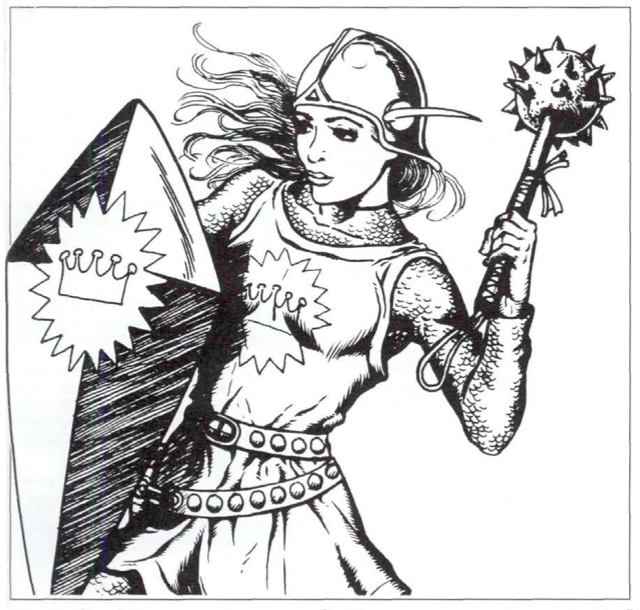
\includegraphics[width=0.7\textwidth,keepaspectratio]{ogCleric.png}\par
\vspace{0.4cm}
{\itshape Legends say the magic of healing was the first learned by
mortals.}\par
\vspace*{\fill}
\end{center}

\end{document}